
% SECTION:
%    transient.tex  
%
% CHAPTER:
%    transients.tex  
%
% ELEVATOR PITCH:
%    Explain in a few sentences what the relevant discovery or
%    measurement is going to be discussed, and what will be important
%    about it. This is for the browsing reader to get a quick feel
%    for what this section is about.
%
% COMMENTS:
%
%
% BUGS:
%
%
% AUTHORS:
%  Stefano Valenti , Federica Bianco (@fedhere)
%
% ====================================================================

\section{Realtime Identification of Young Transients}
\def\secname{\chpname:transientsAge}\label{sec:\secname}


\credit{svalenti}, \credit{fedhere} % (Writing team)

For many transients, the first few hours after event beginning reveal a tremendous amount of fundamental information. A large number of resources in the transient community are devoted to the study of the very early phases of transients (e.g. SNe, GRBs). Since real-time discrimination is a very hard task, it is then important to be able to select, among the large number of transients discovered by LSST, the youngest objects, in order to devise follow-up plans and best distribute precious follow-up resources. In this section we investigate the feasibility of identification of young transients from the LSST data alone, using the intra-night visits.

The Baseline Cadence~\opsimdbref{db:baseCadence} predicts that, on average,
fields in the main survey are revisited every $\sim3$ days in any filter
(\autoref{fig:enigmaGapAll}), and every $\sim15$ days when using only
$r$ band visits (\autoref{fig:enigmaGapr}).  Hence, we are most likely
to discover faint transients that are within 3 days of peak brightness.
However, for the small subset of nearby events, we can hope to discover
them within a few days of explosion.  The challenge is to discriminate
these truly young events from newly-discovered SN that are near peak
brightness.
Within the~\opsimdbref{db:baseCadence} cadence, and most cadences
realized thus far, the second intra-night visit occurs around 30
after the first visit (to maximize the Solar System
moving objects recovery,~\autoref{chp:solarsystem}). We want to understand {\bf\emph{how the intra-night gap enables, affects, and can be used to maximize the identification of new transients as young}}, where, by young, we mean within a day of outburst/explosion.

To begin to answer this question, we limit our investigation to light curve shape in just the r band, and specifically to what can be done in $r$ band. We have selected a representative set of transients with good photometric coverage in the first week after the the outburst/explosion (left panel of \autoref{fig:earlyslope}) and computed the light curve slope as a function of time in magnitudes per day (right panel of \autoref{fig:earlyslope}). In \autoref{fig:earlyrise} we report the change in $r$ brightness between the first and the second visit for the same set of transients as function of phase.

Despite the heterogeneity in light curve shapes, most of the transients show a similar change in brightness on short time scales. 
This confirms that early classification of the transient sub-type is a
major challenge. However, since in general young transients show a fast
increase in brightness, it is much easier to assess whether a transient is
\emph{young}.  Simply put, young transients will show a much larger
brightness change between visits than old events.
This discrimination is aided by a larger time gap between visits (e.g. 2 hours).
Within 30 minutes the change in brightness is of the order of $1\%$, or
even less, for most transients even within the first $\sim3$ days from the
start of the outburst/explosion (\autoref{fig:earlyslope}, left). Thus a
measurement of the change would require a $SNR\gtrsim500$ on each
measurement. Longer gaps give us more leverage: with a time gap of
$\sim2$~hours after the first visit, the change of brightness will increase
to $\sim5\%$. However the breadth of the gap is not unlimited: a gap of 24
hours imposes a significant delay in triggering follow up for these
fast-evolving events.

A natural metric to compare cadences for this purpose 
is the median time difference between
the first and last observations of a field each night.  This differs from
the \texttt{IntraNightGapsMetric}, as the latter only compares consecutive
observations of a field and hence underestimates the nightly time baseline
when there are three or more observations of a field in a night.

The classification of interesting transients, at an early stage, can be
aided by using supplementary information, such as historical information
from previous visits, and by color information about the transient. But to
properly assess the color of an evolving transient, the
gap between observations in different filters should not exceed a few hours 
(\autoref{sec:\chpname:SNtransients}).

Finally, we stress that the quality and completeness of early
multiwavelengh data available at this time is limited. The sample of
astronomical transients used here is not comprehensive, and a uniform
set of homogeneous data of different transients is still needed in
order to further investigate the ideal separation between
observations, the need for color information, and the tension between
the two.

{\bf\emph{In the light of these considerations, we recommend the
    simulation of a cadence with three visits per field, per night,
    two in the same band, but spaced by two hours or more, and a third
    in a different band. This criteria could be limited to the
    observations above and below the ecliptic plane, where recovery of
    Solar System objects puts less strain on the cadence
    requirements. }}

{\bf\emph{Furthermore, we note that the currently envisioned
    deep drilling cadence prioritizes depth per visit at the expense
    of a higher cadence. One hour per night on a deep drilling field
    reaches a depth that not required for almost all transient science
    cases, and by cycling to a different field each night, the time
    between visits for a particular field is too long for many
    important science cases. Even with higher overhead, a more useful
    approach for nearly all transient sciene, that the deep drilling
    fields are designed to facilitate, would be to observe 3 or 4 of
    the available fields each night for 15 or 20 minutes.}}

\begin{figure}[hbt]
\centerline{
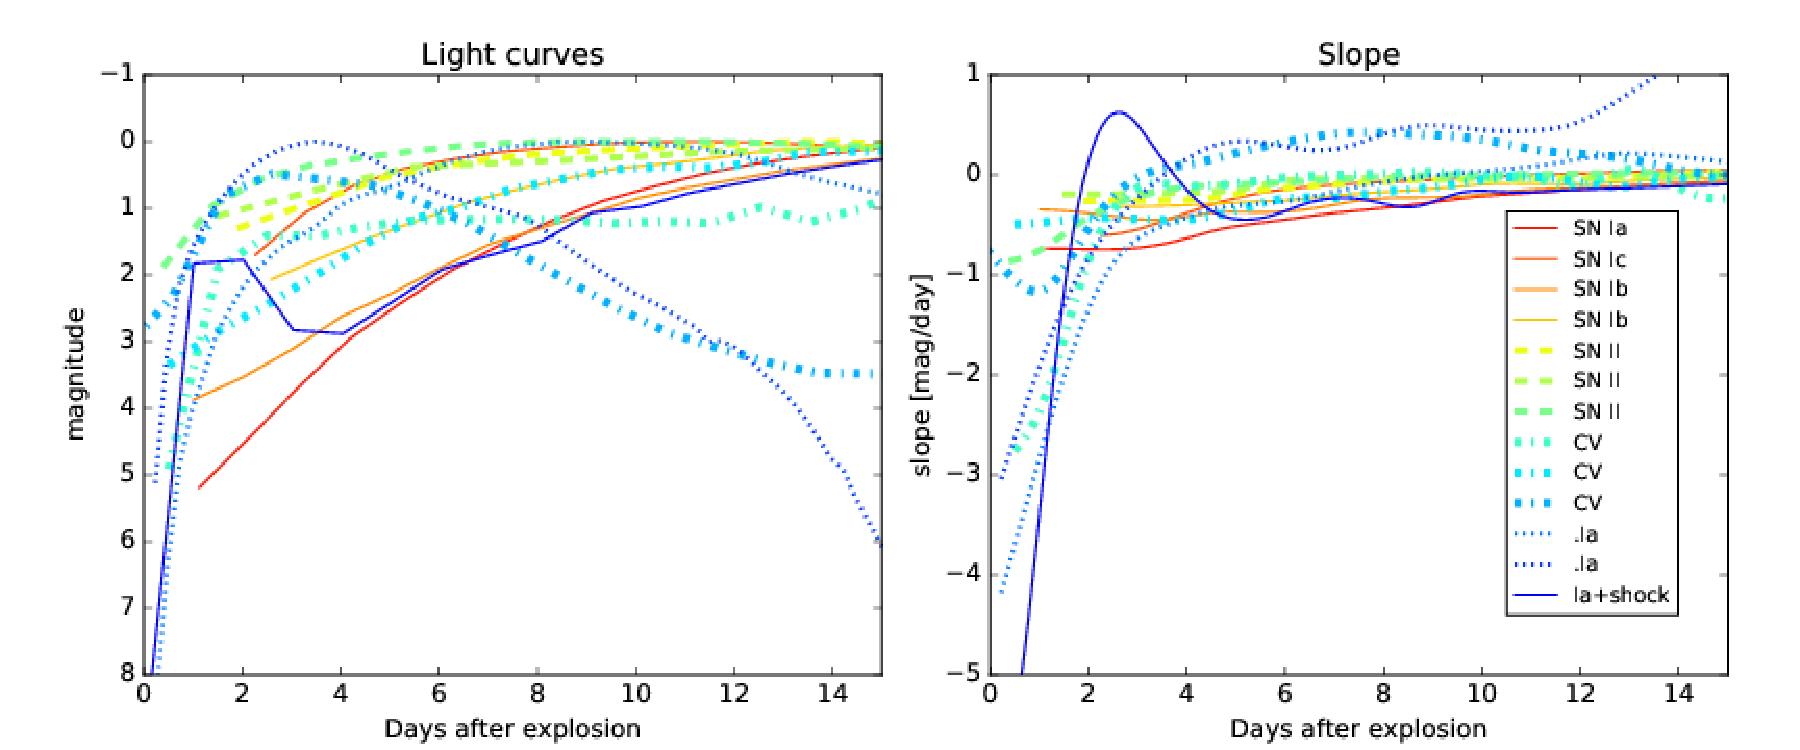
\includegraphics[width=\textwidth]{figs/transients/earlyslope1.pdf}
}
\caption{\emph{Left}: $r'$-band light curve for representative transients as function of the phase from the beginning of the transient outburst/explosion for the first few days of the transient life. \emph{Right}: slope of the transient evolution. Data from: SN~Ia,~\citet{Olling15}; SNII,~\citet{Rubin16}; SN~.Ia,~\citet{Shen10}; SN~Ib,~\citet{Valenti11},~\citet{Cao13}; SN~Ic,~\citet{Mazzali02}; CV, ~\citet{Sokoloski13}, Finzell et al. (in prep), SN~Ia+interaction (see~\autoref{sec:\chpname:SNtransients})}.
\label{fig:earlyslope}
\end{figure}

\begin{figure}[hbt]
\centerline{
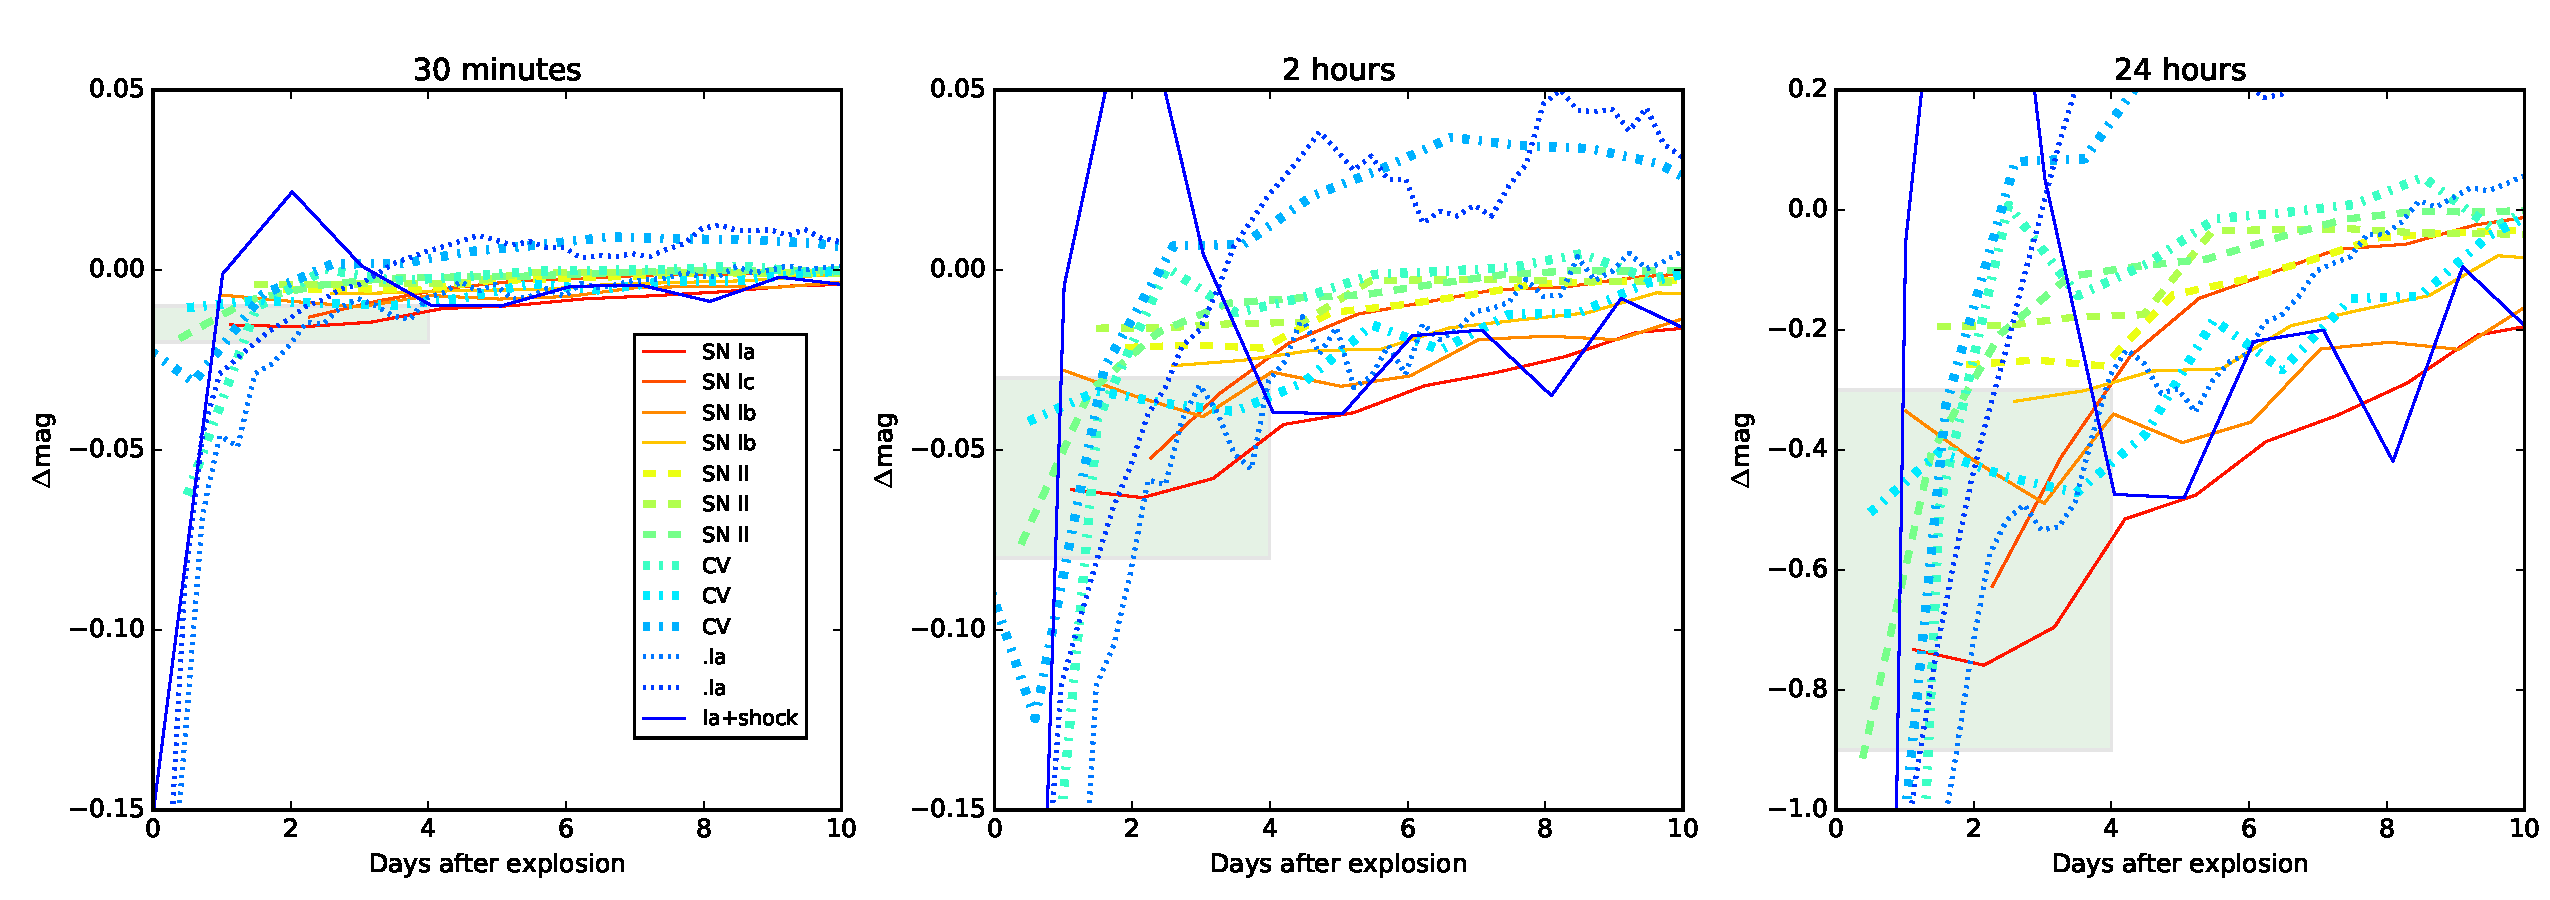
\includegraphics[width=\textwidth]{figs/transients/earlyrise1.pdf}
}
\caption{Observed magnitude change between two consecutive observations for a representative set of astronomical transients, as a function of the phase. We consider observation gaps of 30 minutes  (left panel), 2 hours (central panel) and 24 hours (right panel). 
}
\label{fig:earlyrise}
\end{figure}
